\chapter{Metodologia}

Neste capítulo especificamos os métodos e as técnicas utilizadas para responder se é possível, 
através de \textit{Sequence Design}, 
projetar uma proteína que desempenhe a mesma função do FIX, mas com maior estabilidade e menor
imunogenicidade. Para responder a esta pergunta, foram estabelecidos os seguintes objetivos:

\begin{enumerate}
  \item Desenvolver um \textit{pipeline} genérico que produza sequências que mimetizem uma estrutura qualquer.
  \item Obter um conjunto de sequências de aminoácidos que se conformam em estruturas similares ao FIX baseado na métrica \textit{TMScore}.
  \item Avaliar, dentro do conjunto de proteínas obtidas em 1, quais possuem potencial de substituir o FIX de modo tornar o tratamento de Hemofilia tipo B mais acessível e eficiente.
\end{enumerate}

\section{Estrutura do pipeline}

De modo a atender os objetivos citados, propusemos um \textit{pipeline} de \textit{Sequence Design} genérico, 
cuja entrada é uma estrutura proteíca alvo e a saída 
é um conjunto de sequências que mimetizam a estrutura de entrada. 

A estrutura alvo utilizada é o domínio protease do FIX humano.
O arquivo contendo as coordenadas tridimensionais dessa estrutura foi preparado 
em condições simuladas compatíveis com o ambiente fisiológico, isto é, meio aquoso,
temperatura de $37\,^\circ\mathrm{C}$ e pH neutro. Essa estrutura foi disponibilizada pelo trabalho de \cite{CS}.

O \textit{pipeline}, ilustrado na figura \ref{fig:proposta}, foi implementado de forma modular, 
sendo composto por três módulos principais: Condições Iniciais; 
Treinamento e Geração de Sequências.

No módulo de Condições Iniciais obtemos a sequência inicial de aminoácidos
utilizando o \textit{ProteinMPNN}\footnote{Disponível em: \url{https://github.com/dauparas/ProteinMPNN/}},
adotado como heurística \( H \).
Esse modelo é uma rede neural profunda baseada em grafos, 
que recebe como entrada uma estrutura tridimensional 
e prediz a sequência mais provável de se conformar àquela estrutura, 
com base na orientação espacial dos átomos (\cite{ProteinMPNN}).
Definimos o \textit{ProteinMPNN} como heurística por apresentar 
desempenho superior a métodos clássicos, como \textit{Rosetta}, 
em diversas métricas de reconstrução de sequência a partir da estrutura, 
incluindo taxa de recuperação e viabilidade estrutural (\cite{ProteinMPNN}).

No módulo de Treinamento, uma rede neural profunda, o \textit{GenSeq}, é treinada para atuar como o Agente $A$,
sendo capaz de realizar mutações que otimizam a similaridade com a estrutura alvo, isto é, o FIX.
O \textit{GenSeq} será treinado utilizando um algoritmo de aprendizado por reforço profundo, 
o \textit{Proximal Policy Optimization} (PPO\footnote{Disponível em: \url{https://stable-baselines3.readthedocs.io/en/master/modules/ppo.html}}) (\cite{PPO}).
Para ser processada pela rede neural, a sequência de entrada é convertida em um vetor de \textit{embeddings},
que é construído via MDS\footnote{Disponível em: \url{https://scikit-learn.org/0.16/modules/generated/sklearn.manifold.MDS.html}} (\textit{Multidimensional Scaling}) 
a partir da matriz de distâncias entre 
os aminoácidos, obtida a partir do trabalho de \cite{aminodist}, 
detalhado em \ref{subsection:AminoDist}.

O treinamento é realizado em dois estágios. No primeiro estágio o objetivo é restringir o espaço de ações do agente 
de modo a orientá-lo a evitar mutações em regiões altamente conservadas da sequência e 
substituições entre aminoácidos com perfis bioquímicos muito distintos. 
A função objetivo $F_{\text{obj}}$ neste estágio é definida como uma relação 
entre o grau de conservação de cada posição na sequência — obtido a partir do trabalho de \cite{CS} e detalhado em \ref{subsection:CS} — e a similaridade entre aminoácidos, 
medida com base em uma matriz de distâncias desenvolvida em \cite{aminodist}. 

No segundo estágio, o \textit{GenSeq} é orientado a realizar mutações que otimizam outra 
função objetivo: a similaridade entre a estrutura predita e a alvo. 
Para predizer a estrutura tridimensional resultante de uma sequência mutada,
utilizamos o \textit{ESMFold}\footnote{Modelo consumido via API: \url{https://api.esmatlas.com/foldSequence/v1/pdb/}},
um modelo baseado em \textit{transformers} capaz de realizar a predição de estruturas proteicas 
a partir de sequências de aminoácidos (\cite{ESMFold}). 
Para viabilizar o \textit{pipeline}, optamos por este modelo principalmente devido 
a sua elevada velocidade de predição, que é cerca de uma ordem de grandeza maior que 
outros modelos \textit{benchmarking}, como o \textit{AlphaFold} (\cite{ESMFold}).
A similaridade estrutural entre a estrutura predita e a estrutura alvo 
é avaliada com a métrica \textit{TMScore}, 
selecionada por sua robustez na avaliação da similaridade estrutural global 
e por oferecer valores normalizados entre 0 e 1, 
o que facilita a interpretação dos resultados. 
O cálculo do \textit{TMScore} é realizado por meio da plataforma \textit{US-align} (\cite{USalign}).

Por fim, no módulo de Geração de Sequências, 
o agente treinado é utilizado para produzir um conjunto de variantes proteicas estruturalmente semelhantes ao FIX,
por meio de um processo de mutação orientado. 
As sequências geradas são avaliadas para identificar candidatas viáveis 
a substituir o FIX no tratamento da hemofilia tipo B.

\begin{figure}[H]
  \centering
  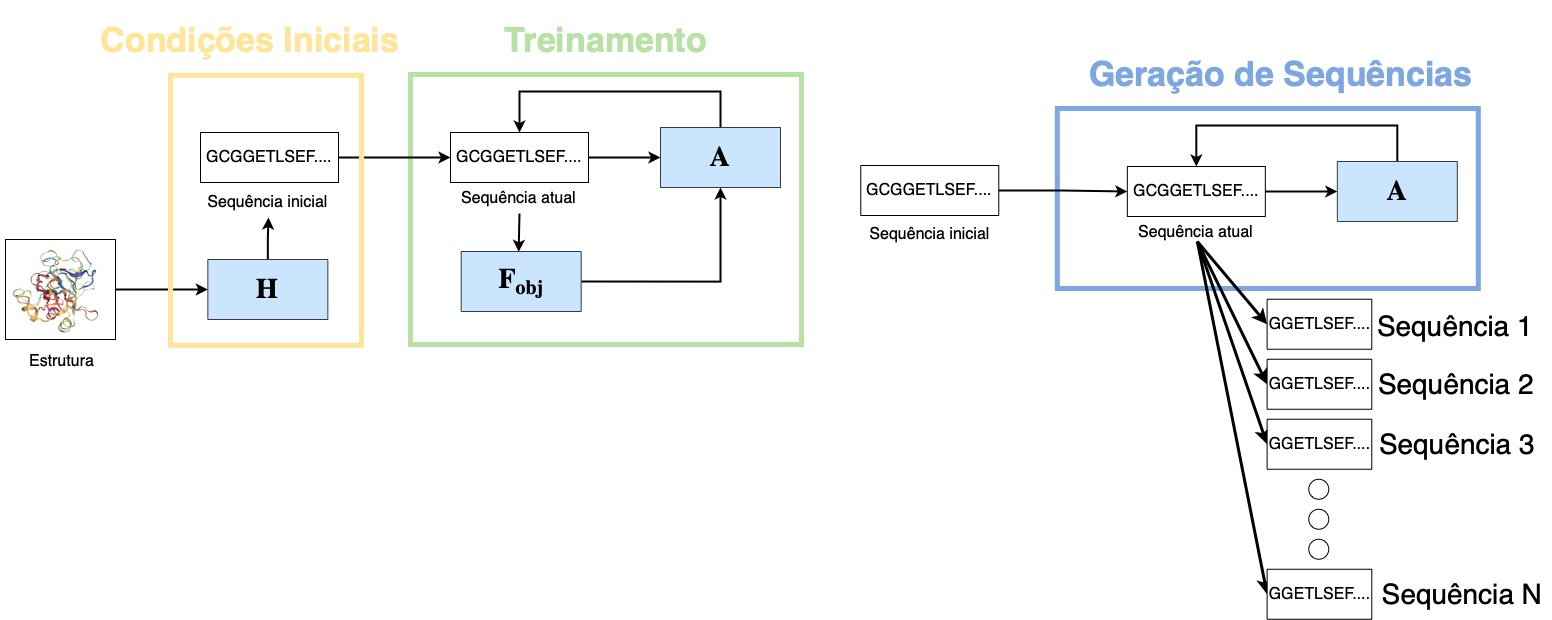
\includegraphics[width=.8\textwidth]{figuras/metodologia-pipeline_proposta.jpg}
  \caption{\textit{Pipeline} proposto de \textit{Sequence Design}.}
  \label{fig:proposta}
\end{figure}


\section{Métodos de avaliação}

A avaliação das proteínas geradas pelo agente é realizada em três etapas: 
análise estrutural, interação molecular por \textit{Docking} e imunogenicidade. 
Cada etapa é essencial para verificar se as proteínas geradas possuem características estruturais, 
funcionais e imunológicas adequadas para substituir o FIX no tratamento da hemofilia B.  

A primeira etapa consiste em medir a similaridade estrutural entre cada proteína gerada
e o FIX por meio do \textit{TMScore}. 
São selecionadas apenas proteínas com \textit{TMScore} superior a 92\%.

Na segunda etapa, avaliamos a capacidade das proteínas geradas de desempenhar a função do FIX, 
isto é, interagir com o Fator VIII (FVIII) e formar o complexo tenase, conforme descrito em \ref{subsection:FIX}.
Assim como o FIX, o arquivo contendo as coordenadas tridimensionais do FVIII foi disponibilizada por \cite{CS} 
considerando meio aquoso, temperatura de $37\,^\circ\mathrm{C}$ e pH neutro. 

De modo a viabilizar a análise da iteração com o FVIII, 
é necessário alinhar estruturalmente a proteína gerada com o FVIII
para garantir que a proteína mutante ocupe a mesma posição relativa do FIX no complexo original. 
Isso é feito utilizando \textit{ChimeraX} (\cite{ChimeraX}) por meio do comando \texttt{matchmaker}.

\begin{figure}[H]
  \centering
  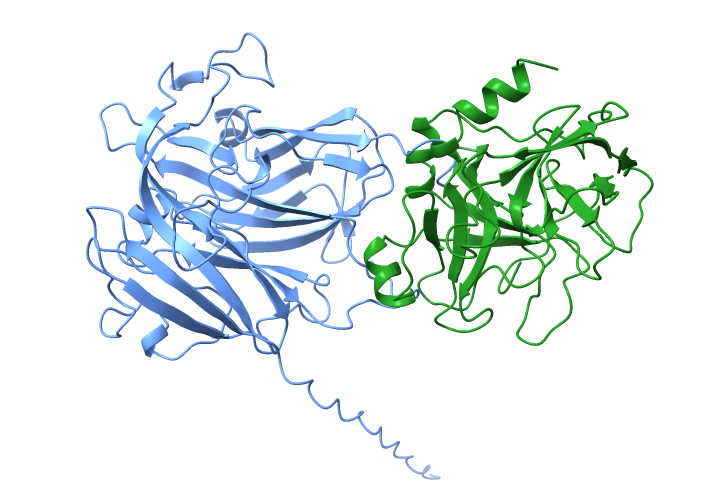
\includegraphics[width=.6\textwidth]{figuras/complexocomid63.png}
  \caption{Proteína gerada 63 (verde) alinhada com o FVIII (azul)}
\end{figure}

Após o alinhamento estrutural, realizamos o \textit{docking molecular} 
por meio do protocolo \textit{Rosetta Docking}\footnote{Disponível em: \url{https://docs.rosettacommons.org/docs/latest/application_documentation/docking/docking-protocol}}, 
que permite prever a orientação e estabilidade do complexo proteína-proteína gerado.
O \textit{Rosetta Docking} consiste em um procedimento iterativo que busca a conformação de menor energia livre do complexo.
O protocolo inicia com a geração de múltiplas poses, onde a proteína mutante é rotacionada e transladada em relação ao FVIII.
Em seguida, as conformações passam por um refinamento energético que inclui otimização da 
orientação relativa (\textit{rigid-body minimization}) e ajuste das cadeias laterais na interface 
(\textit{side-chain minimization}). 
O protocolo utiliza a função de energia do \textit{Rosetta} para estimar a estabilidade do complexo,
considerando fatores como interações de \textit{Van der Waals}, 
ligações de hidrogênio, energia eletrostática e solubilidade.
Baseado na função de energia e da posição relativa dos átomos no complexo, 
é calculada as métricas 
\textit{Contact Molecular Surface} (CMS), 
\textit{Interface Buried SASA} (IBSASA), 
\textit{Delta Gibbs Free Energy of Binding} (DDG) e
\textit{Surface Area Potential Score} (SAP Score), detalhadas em \ref{subsection:Docking}.
A partir dessas métricas é possível avaliar de forma quantitativa 
se as proteínas geradas possuem uma interação favorável com o FVIII, ou seja, 
são capazes de desempenhar a função do FIX.

A terceira e última etapa de avaliação consiste na análise da imunogenicidade das proteínas geradas.
O objetivo desta etapa é identificar possíveis epítopos imunogênicos presentes nas sequências, 
os quais poderiam desencadear respostas imunes indesejadas nos pacientes.
Esses epítopos são regiões da sequência que se ligam a moléculas do 
Complexo Principal de Histocompatibilidade de classe II (MHC II) (vide \ref{subsection:RespImuno}). 
Para realizar esta análise, foi utilizado o \textit{NetMHCIIpan} versão 4.1 (\cite{Jensen2018NetMHCIIpan}), 
algoritmo desenvolvido para predição de ligação de peptídeos a moléculas 
de MHC II. 
O \textit{NetMHCIIpan} emprega técnicas de aprendizado de máquina para prever a afinidade de ligação de peptídeos 
derivados das proteínas analisadas às diferentes variantes alélicas de MHC II. 
Quanto mais peptídeos propensos a se ligar a alelos de MHC II,
maior a probabilidade de desencadear uma resposta imune.

Para esta análise foram utilizados 46 alelos de MHC II frequentes na população humana, 
pertencentes aos grupos DP, DQ, DRB1 DRB3, DRB4 e DRB5.
Estes alelos foram selecionados com o intuito de representar a diversidade populacional 
e garantir uma avaliação abrangente da imunogenicidade das variantes propostas.

O número total de epítopos fortes, a afinidade de ligação
e a frequência com que os alelos ocorrem na natureza são as métricas utilizadas
para avaliar e comparar a imunogenicidade das proteínas geradas com a proteína nativa. 




















